\section{Введение}


\subsection{Цель работы}

\begin{enumerate}
    \item Исследовать чувствительность пластин вертикального и горизонтального отклонений осциллографической трубки.
    \item Наблюдать с помощью осциллографа синусоидальное напряжение, полученное с выхода генератора.
    \item Получить фигуры Лиссажу и определить частоту исследуемого напряжения по фигурам Лиссажу.
\end{enumerate}

\subsection{Решаемые задачи}
\begin{enumerate}
    \item Исследовать чувствительность пластин вертикального и горизонтального отклонений осциллографической трубки. 
    \item Наблюдать с помощью осциллографа синусоидальное напряжение, полученное с выхода генератора. 
    \item Получить фигуры Лиссажу и определить частоту исследуемого напряжения по фигурам Лиссажу. 
\end{enumerate}

\section{Основная часть} 


\subsection{Эксперимент}

\textbf{Блок схема осцилографа}

\begin{figure}[H]
\centering
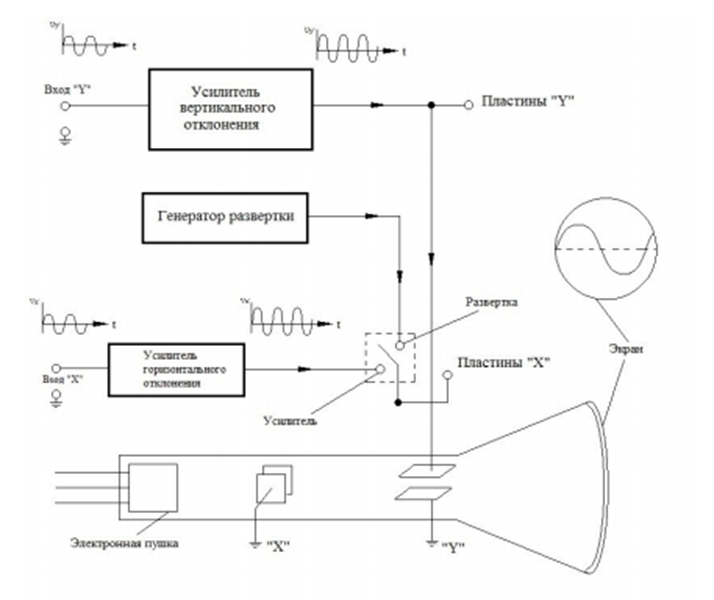
\includegraphics[width=0.9\textwidth]{image1.png}
\caption{Блок схема осцилографа}
\label{fig:distribution}
\end{figure}

\textbf{Схема электрической цепи для исследования чувствительности пластин электронно-лучевой трубки}

\begin{figure}[H]
\centering
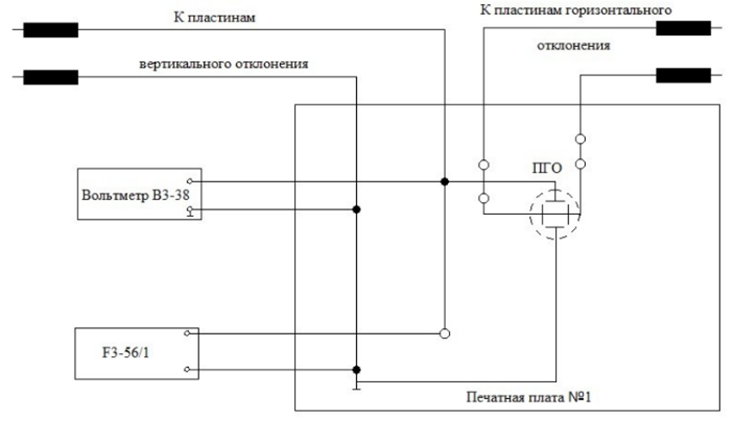
\includegraphics[width=0.9\textwidth]{image2.png}
\caption{Схема электрической цепи для исследования чувствительности пластин электронно-лучевой трубки}
\label{fig:distribution}
\end{figure}

\textbf{Схема электрической цепи для получения фигур Лиссажу и измерения частоты синусоидального сигнала}

\begin{figure}[H]
\centering
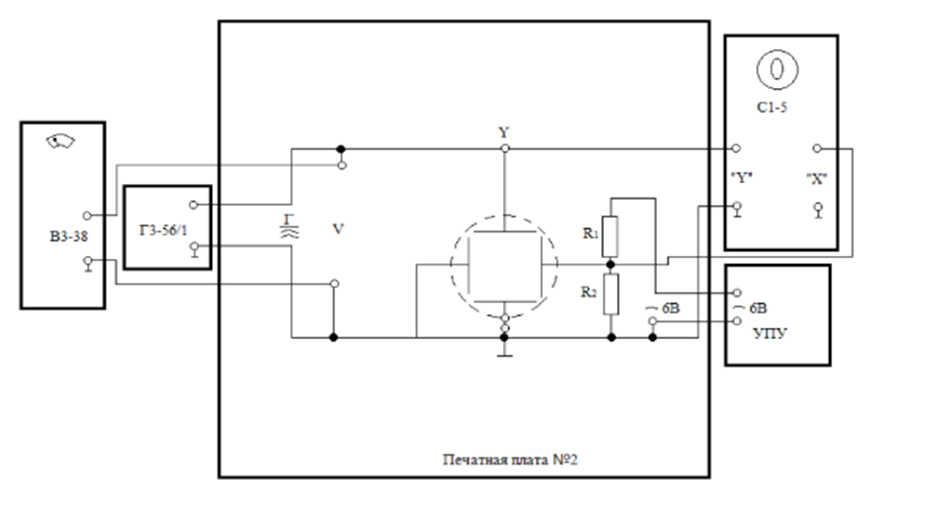
\includegraphics[width=0.9\textwidth]{image3.png}
\caption{Схема электрической цепи для получения фигур Лиссажу и измерения частоты синусоидального сигнала}
\label{fig:distribution}
\end{figure}



\subsection{Обработка данных и обсуждение результатов}

\subsubsection{Таблицы}

Исследование чувствительности пластин осциллографической трубки. Формула для расчета чувствительности (как горизонтального, так и вертикального отклонений, а также для самого осциллографа):

\[
S = \frac{L}{2\sqrt{2}U_{eff}}
\]

\begin{table}[H]
\centering
\caption{Пластины вертикального отклонения (ПВО)}
\label{tab:pvo}
\begin{tabular}{|c|c|c|c|}
\hline
Длина & Эффективное напряжение & Чувствительность \\
(мм) & (В) & (мм/В) \\
\hline
10 & 3,0 & 1,1785 \\
\hline
20 & 7,0 & 1,0102 \\
\hline
30 & 11,0 & 0,9642 \\
\hline
40 & 15,5 & 0,9124 \\
\hline
50 & 19,5 & 0,9065 \\
\hline
\end{tabular}
\end{table}

\begin{table}[H]
\centering
\caption{Пластины горизонтального отклонения (ПГО)}
\label{tab:pgo}
\begin{tabular}{|c|c|c|c|}
\hline
Длина & Эффективное напряжение & Чувствительность \\
(мм) & (В) & (мм/В) \\
\hline
10 & 3,5 & 1,0102 \\
\hline
20 & 7,7 & 0,9186 \\
\hline
30 & 12,5 & 0,8485 \\
\hline
40 & 17,5 & 0,8081 \\
\hline
50 & 22,0 & 0,8036 \\
\hline
\end{tabular}
\end{table}

\begin{table}[H]
\centering
\caption{Максимальная чувствительность осциллографа}
\label{tab:distribution}
\begin{tabular}{|c|c|c|c|}
\hline
Длина & Эффективное напряжение & Чувствительность \\
(мм) & (В) & (мм/В) \\
\hline
10 & 0,0036 & 982,4088 \\
\hline
20 & 0,0069 & 1024,8487 \\
\hline
30 & 0,0110 & 964,1978 \\
\hline
40 & 0,0150 & 942,8090 \\
\hline
50 & 0,0185 & 955,8077 \\
\hline
\end{tabular}
\end{table}



\begin{table}[H]
\centering
\caption{Измерение известной частоты при наблюдении фигур Лиссажу}
\label{tab:distribution}
\begin{tabular}{|c|c|c|c|c|}
\hline
Вид фигуры Лиссажу & 0 & 8 & 000 & $\infty$ \\
\hline
Отношение частот $f_x / f_y$ & 1:1 & 2:1 & 1:3 & 1:2\\
\hline
Частота по лимбу генератора $f_y$ & 50 & 25 & 150 & 100\\
\hline
Исследуемая частота $f_x$ & 50 & 50 & 50 & 50\\
\hline
\end{tabular}
\end{table}

\subsection*{Определение чувствительности пластин осциллографа}

Средние значения чувствительности пластин вертикального и горизонтального отклонений рассчитывались по формуле:
\[
\overline{S} = \frac{\sum_{i=1}^{n} S_i}{n}
\]
где $S_i$ — значение чувствительности пластин в полученных точках, $n$ — количество значений.

Таким образом получаем средние значения чувствительности пластин:
\[
\overline{S_y} = 0,3826 \text{ мм/В}
\]
\[
\overline{S_x} = 0,2869 \text{ мм/В}
\]

Поиск погрешностей (с учетом, что берем $n = 4$ для ПГО и $n = 5$ для ПВО):
\[
\sigma_{\overline{x}} = \sqrt{\frac{\sum_{i=1}^{n} d_i^2}{n(n-1)}}
\]
где $d_i = x_i - \overline{x}$.

Итак, имеем:
\[
\sigma_{\overline{S_y}} = 0,0043, \quad S_y = 0,3826 \pm 0,0043 \text{ мм/В}
\]
\[
\sigma_{\overline{S_x}} = 0,0232, \quad S_x = 0,2869 \pm 0,0232 \text{ мм/В}
\]


\subsection*{Расчёт для пластин вертикального отклонения (ПВО)}
Из предыдущих данных среднее значение чувствительности на участке постоянной чувствительности:
\[
S_y = 0,9277 \text{ мм/В}
\]

Максимальная чувствительность (при $L = 10$ мм, $U_{\text{eff}} = 3,0$ В):
\[
(S_y)_m = 1,1785 \text{ мм/В}
\]

Максимальный коэффициент усиления:
\[
K_m = \frac{(S_y)_m}{S_y} = \frac{1,1785}{0,9277} = 1,270
\]

\subsection*{Среднее значение частоты f_x}

Среднее значение частоты fx синусоидального напряжения, измеренное по фигурам Лиссажу, оказалось равным 50 Гц для каждой из рассмотренных в опыте фигур.

\subsubsection{Графики}

\begin{figure}[H]
\centering
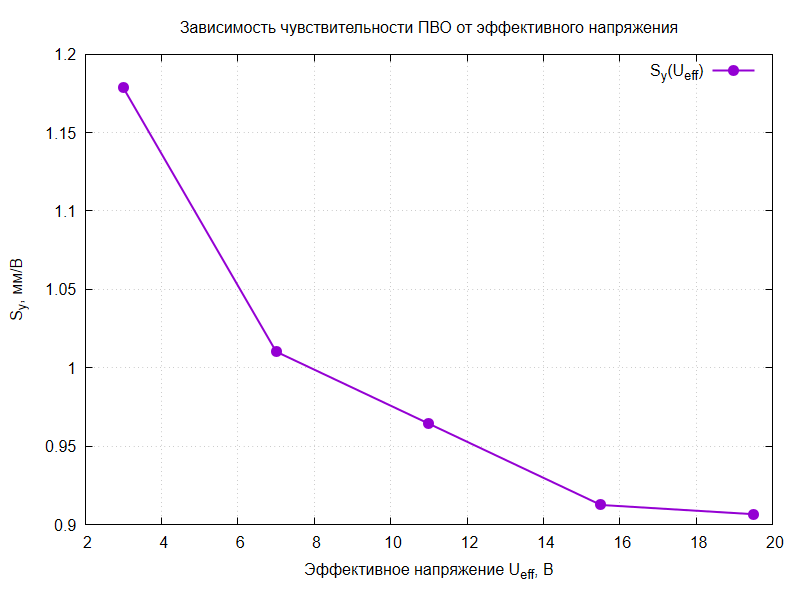
\includegraphics[width=0.9\textwidth]{pvo_graph.png}
\caption{Зависимость чувствительности ПВО от эффективного напряжения}
\label{fig:drift}
\end{figure}


\begin{figure}[H]
\centering
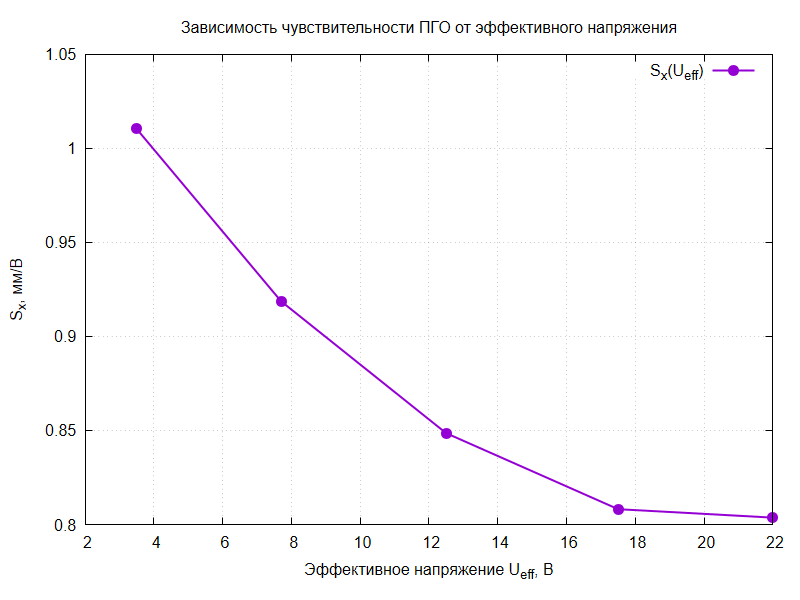
\includegraphics[width=0.9\textwidth]{pgo_graph.png}
\caption{Зависимость чувствительности ПГО от эффективного напряжения}
\label{fig:drift}
\end{figure}

\section{Выводы}
В ходе работы исследована чувствительность пластин вертикального и горизонтального отклонений осциллографической трубки. Установлено, что с ростом эффективного напряжения чувствительность снижается, однако в области высоких напряжений её изменение становится незначительным.

При наблюдении синусоидального напряжения с генератора убедился, что осциллограф корректно отображает форму сигнала.

С помощью фигур Лиссажу определил частоту исследуемого напряжения. Форма фигуры позволяет однозначно установить отношение частот, что даёт возможность точно вычислить неизвестную частоту.

Все задачи, поставленные в работе, выполнены..
